\documentclass[tikz, margin=3.14mm]{standalone}
\usepackage{tikz}
\usepackage{pgfplots}
\pgfplotsset{compat=1.18}

\begin{document}
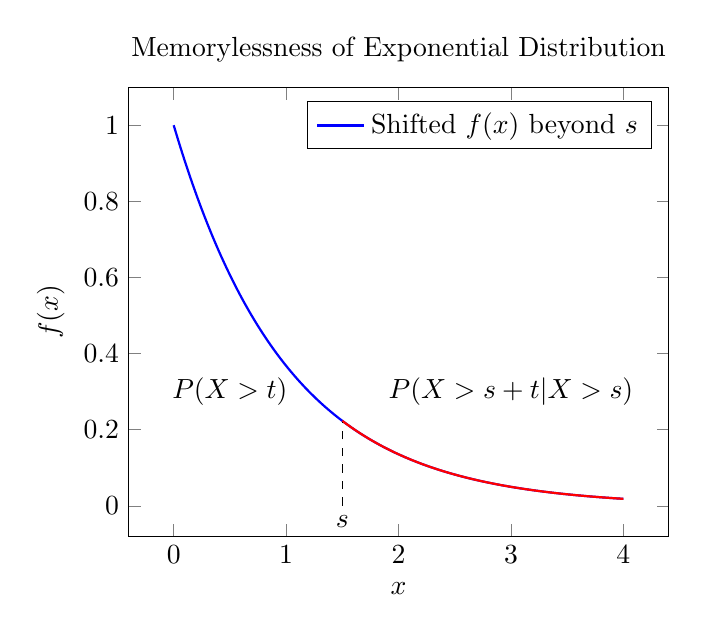
\begin{tikzpicture}
\begin{axis}[
    domain=0:4,
    samples=200,
    xlabel={$x$},
    ylabel={$f(x)$},
    title={Memorylessness of Exponential Distribution},
    legend pos=north east,
    clip=false
]
% Exponential distribution with lambda = 1
\addplot[blue, thick] {exp(-x)};
% \addlegendentry{$f(x)$};

% Highlight the tail distribution beyond s
\def\s{1.5};
\addplot[red, thick, domain=\s:4] {exp(-x+\s)*exp(-\s)};
\addlegendentry{Shifted $f(x)$ beyond $s$};

% Vertical line at s
\draw[dashed] (axis cs:1.5,0) -- (axis cs:1.5,.22);

% Annotations
\node at (axis cs:\s+1.5,0.3) {$P(X > s + t | X > s)$};
\node at (axis cs:0.5,0.3) {$P(X > t)$};
\node[anchor=north] at (axis cs:\s,0) {$s$};
\end{axis}
\end{tikzpicture}
\end{document}
